\documentclass[12pt]{article}

\usepackage{graphicx}
\usepackage{listings}
\usepackage[a4paper, total={6in, 10in}]{geometry}
\usepackage{hyperref}
\title{Your Report Title Here}
\author{Your Name}
\date{\today}

\begin{document}

    \maketitle


    \section{Analysis of Original Application}

    \subsection{Description}
    The original application selected for this project was the implementation of the Merge Sort
    algorithm in C\#. Merge Sort is a renowned divide-and-conquer sorting algorithm that
    recursively divides an array into two halves, sorts each half, and merges them back in a
    sorted order. This algorithm was chosen because of its computational intensity, especially
    when dealing with substantial datasets. Its time complexity, $O(n \log n)$, can be relatively
    slow for large datasets. The divide-and-conquer nature of the Merge Sort algorithm, 
    inherently, makes it a promising candidate for parallelization. Given the potential, the 
    goal was to harness parallel processing capabilities to enhance the sorting speed and reduce
    execution time.

    This specific sequential version of Merge Sort was initially implemented from scratch
    for this project and can be found on my \href{https://github.com/CurtisDH/MergeSort}{GitHub}. As a part of CAB301, 
    I had been introduced to this algorithm, which laid a foundation for this project.

    \subsubsection{Two main phases constituted the application's analysis:}
    \begin{itemize}
        \item Profiling the Sequential Implementation: A Stopwatch was integrated to measure the time taken in data generation and sorting, providing concrete metrics to establish the application's baseline performance. The initial version, though functional, had noticeable performance bottlenecks, especially when handling substantial data arrays.
        \item Identifying Potential for Parallelization: Recognizing the computational heft of Merge Sort, especially for expansive datasets, it was hypothesized that sorting various segments of the data array in parallel could drastically decrease the overall execution time. The inherent structure of Merge Sort—its division of data—offered an organic path towards parallelization.
    \end{itemize}

    \subsection{Issues/Bottlenecks Identified}
    \begin{enumerate}
        \item \textbf{Sequential Processing:} The original merge sort algorithm was executed in a sequential manner, which doesn't exploit the potential benefits of modern multi-core processors. Given the divide-and-conquer nature of merge sort, this was a significant area to introduce parallelism for better performance.

        \item \textbf{Recursive Overhead:} The merge sort's recursive nature can lead to additional overhead in managing function calls, especially with larger datasets. Parallel processing can help distribute this load across cores, reducing the time taken per recursion.

        \item \textbf{Data Copying and Merging:} The operation of copying array segments and merging them in the merge sort increases computational overhead. Parallelizing these operations, especially the merge operation, can lead to substantial performance gains.

        \item \textbf{Non-Adaptive Nature:} The original algorithm didn't adapt to the available system resources. An optimized parallel version can be adaptive by determining the number of cores available and then segmenting the data accordingly for concurrent processing.

        \item \textbf{Merging Limitation in Optimized Version:} Despite the introduction of parallelism in the sorting segments in the optimized version, the merging process was still sequential, representing an area that could be further improved through parallel merging techniques.

    \end{enumerate}


    \subsection{Data and Control Dependencies}
    \begin{itemize}
        \item \textbf{Data Dependency:} Discuss any data dependencies that were discovered.
        \item \textbf{Control Dependency:} Discuss any control dependencies that were found.
    \end{itemize}

    \subsection{Before and After Profiling Results}
    \textbf{Before:} Insert detailed profiling results before optimization. \\
    \textbf{After:} Insert detailed profiling results after optimization.


    \section{Use of Tools and Techniques}

    \subsection{Tools Used}
    \begin{enumerate}
        \item Tool 1: Describe how you used this tool.
        \item Tool 2: Describe how you used this tool.
        % Add more items as necessary.
    \end{enumerate}

    \subsection{Techniques Implemented}
    \begin{enumerate}
        \item Technique 1: Discuss the first parallel programming technique you applied.
        \item Technique 2: Discuss the second parallel programming technique you applied.
        % Add more items as necessary.
    \end{enumerate}


    \section{Optimal Speedup}

    \subsection{Description}
    Provide a brief description of how the speedup was achieved.
    \newpage

    \subsection{Speed-up Graph}
    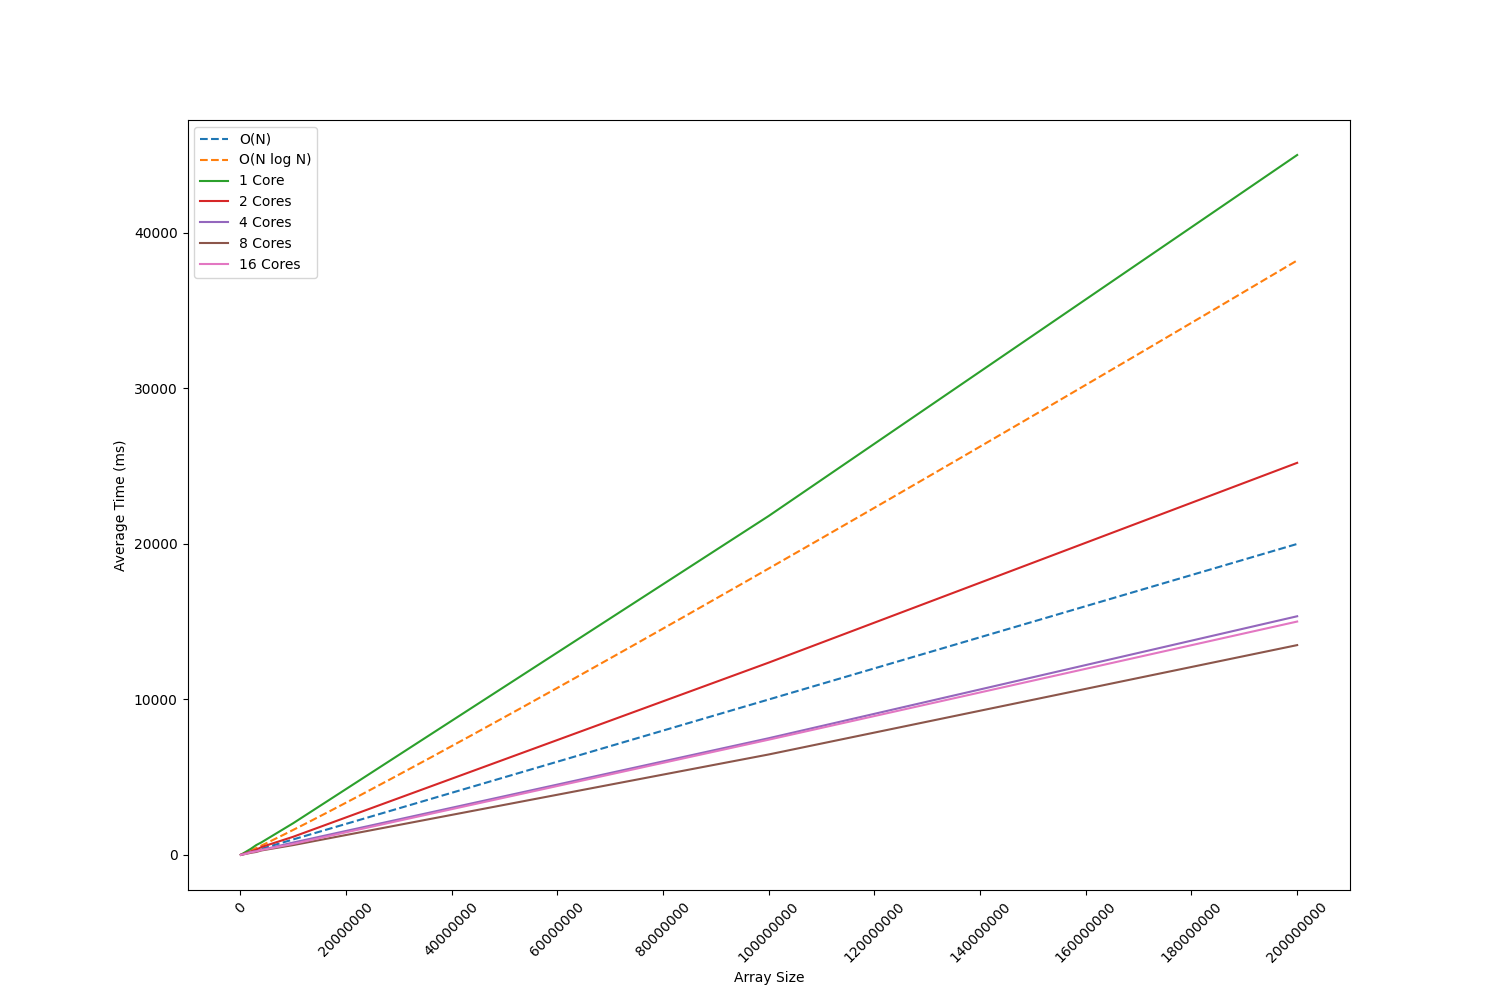
\includegraphics[scale=0.35]{img}

    \subsection{Performance Metrics}
    \textbf{Before Optimization:} Mention metrics such as execution time, throughput, etc. \\
    \textbf{After Optimization:} Mention improved metrics.


    \section{Overcoming Barriers}

    \subsection{Major Barriers Identified}
    \begin{enumerate}
        \item Barrier 1: Describe the first major barrier you faced.
        \item Barrier 2: Describe the second major barrier you faced.
% Add more items as necessary.
    \end{enumerate}

    \subsection{Solutions Implemented}
    \begin{enumerate}
        \item Solution to Barrier 1: Discuss how you overcame the first barrier.
        \item Solution to Barrier 2: Discuss how you overcame the second barrier.
% Add more items as necessary.
    \end{enumerate}

    \subsection{Before and After Code Snippets}
    \begin{lstlisting}
% Insert code snippet before changes.
    \end{lstlisting}

    \begin{lstlisting}
% Insert code snippet after changes.
    \end{lstlisting}


    \section{Report}

    \subsection{Introduction}
    Provide a brief introduction to your report.

    \subsection{Body}

    \subsubsection{Section 1}
    Discuss the main content of your report.

    \subsubsection{Section 2}
    Expand on additional findings or insights.
% Add more sections as necessary.

    \subsection{Conclusion}
    Provide a summary of your findings and insights.

    \subsection{Recommendations}
    Provide any recommendations for future improvements or optimizations.

\end{document}
